\documentclass[aspectratio=43]{beamer}
% Theme works only with a 4:3 aspect ratio
\usetheme{CSCS}

\usepackage{tikz}
\usepackage{pgfplots}
\usepackage{pgfplotstable}
\usetikzlibrary{pgfplots.groupplots,spy,patterns}
\usepackage{listings}
\usepackage{color}
\usepackage{tcolorbox}
\usepackage{anyfontsize}
\usepackage{xspace}
\usepackage{graphicx}

% define footer text
\newcommand{\footlinetext}{Introduction to GPUs in HPC}

% Select the image for the title page
\newcommand{\picturetitle}{cscs_images/image5.pdf}

% fonts for maths
\usefonttheme{professionalfonts}
\usefonttheme{serif}

% source code listing
\newcommand{\axpy}{{\ttfamily axpy}\xspace}
\newcommand{\extra}{{\bfseries extra}:\xspace}
%\newcommand{\lst}[1]{\colorbox{white!90!blue}{\lstinline!#1!}}
\newcommand{\lst}[1]{\colorbox{white!20!black}{\lstinline!#1!}}
\newcommand{\lstfont}[1]{\color{#1}\scriptsize\ttfamily}
\newcommand{\lsttinyfont}[1]{\color{#1}\fontsize{7}{7}\ttfamily}
\newcommand{\lstinlinefont}[1]{\color{#1}\scriptsize\ttfamily}

% set indent to a more reasonable level (so that itemize can be used in columns)
\setlength{\leftmargini}{20pt}

%\lstset{
%    language=[ANSI]C++,
%    basicstyle=\lstinlinefont{blue!30!black},
%    breaklines=true
%}
\lstdefinestyle{terminal}{
    showstringspaces=false,
    backgroundcolor=\color{white},
    basicstyle=\lstfont{black},
    identifierstyle=\lstfont{black},
    keywordstyle=\lstfont{black},
    numberstyle=\lstfont{black},
    stringstyle=\lstfont{black},
    commentstyle=\lstfont{black},
    emph={
        aprun, make
    },
    emphstyle={\lstfont{black}},
    breaklines=true
}

\lstset{
    language=[ANSI]C++,
    showstringspaces=false,
    backgroundcolor=\color{white!10!black},
    basicstyle=\lstfont{white},
    identifierstyle=\lstfont{white},
    keywordstyle=\lstfont{magenta!40!white},
    numberstyle=\lstfont{white},
    stringstyle=\lstfont{cyan},
    commentstyle=\lstfont{yellow!30!white},
    moredelim=[is][\lstfont{green!60!white}]{@}{@},
    emph={
        cudaMalloc, cudaFree,
        cudaMallocHost, cudaFreeHost,
        cudaMemcpyAsync, cudaMemcpy, cudaMemcpyHostToDevice, cudaMemcpyDeviceToHost,
        cudaSuccess, cudaGetLastError, cudaGetErrorString,
        cudaErrorMemoryAllocation, cudaError_t,
        cudaOccupancyMaxPotentialBlockSize,
        __global__, __shared__, __device__, __host__,
        __syncthreads,
        cudaEvent_t, cudaStream_t,
        cudaEventCreate, cudaEventSynchronize, cudaEventDestroy,
        cudaEventElapsedTime, cudaEventQuery, cudaEventRecord,
        cudaStreamWaitEvent,
        threadIdx, blockIdx, blockDim, gridDim,
        cudaStream_t, cudaStreamCreate, cudaStreamDestroy,
        \<\<\<,
    },
    emphstyle={\lstfont{green!60!white}},
    breaklines=true
}

\definecolor{codenumber}{rgb}{0.5,0.5,0.5}
\definecolor{codekeyword}{rgb}{0.9,0.4,0.7}
\definecolor{codeCUDA}{rgb}{1.0,0.6,0.6}

\lstdefinestyle{boxcuda}{
    language=[ANSI]C++,
    showstringspaces=false,
    backgroundcolor=\color{white!10!black},
    basicstyle=\lstfont{white},
    identifierstyle=\lstfont{white},
    keywordstyle=\lstfont{magenta!40!white},
    numberstyle=\lstfont{white},
    stringstyle=\lstfont{cyan},
    commentstyle=\lstfont{yellow!30!white},
    moredelim=[is][\lstfont{green!60!white}]{@}{@},
    emph={
        cudaMalloc, cudaFree,
        cudaMallocHost, cudaFreeHost,
        cudaMemcpyAsync, cudaMemcpy, cudaMemcpyHostToDevice, cudaMemcpyDeviceToHost,
        cudaSuccess, cudaGetLastError, cudaGetErrorString,
        cudaErrorMemoryAllocation, cudaError_t,
        cudaOccupancyMaxPotentialBlockSize,
        __global__, __shared__, __device__, __host__,
        __syncthreads,
        cudaEvent_t, cudaStream_t,
        cudaEventCreate, cudaEventSynchronize, cudaEventDestroy,
        cudaEventElapsedTime, cudaEventQuery, cudaEventRecord,
        cudaStreamWaitEvent,
        threadIdx, blockIdx, blockDim, gridDim,
        cudaStream_t, cudaStreamCreate, cudaStreamDestroy,
        \<\<\<,
    },
    emphstyle={\lstfont{green!60!white}},
    breaklines=true
}

\lstdefinestyle{boxcudatiny}{
    language=[ANSI]C++,
    showstringspaces=false,
    backgroundcolor=\color{white!10!black},
    basicstyle=\lsttinyfont{white},
    identifierstyle=\lsttinyfont{white},
    keywordstyle=\lsttinyfont{magenta!40!white},
    numberstyle=\lsttinyfont{white},
    stringstyle=\lsttinyfont{cyan},
    commentstyle=\lsttinyfont{yellow!30!white},
    moredelim=[is][\lsttinyfont{green!60!white}]{@}{@},
    emph={
        cudaMalloc, cudaFree,
        cudaMallocHost, cudaFreeHost,
        cudaMemcpyAsync, cudaMemcpy, cudaMemcpyHostToDevice, cudaMemcpyDeviceToHost,
        cudaSuccess, cudaGetLastError, cudaGetErrorString,
        cudaErrorMemoryAllocation, cudaError_t,
        cudaOccupancyMaxPotentialBlockSize,
        __global__, __shared__, __device__, __host__,
        __syncthreads,
        cudaEvent_t, cudaStream_t,
        cudaEventCreate, cudaEventSynchronize, cudaEventDestroy,
        cudaEventElapsedTime, cudaEventQuery, cudaEventRecord,
        cudaStreamWaitEvent,
        threadIdx, blockIdx, blockDim, gridDim,
        cudaStream_t, cudaStreamCreate, cudaStreamDestroy,
    },
    emphstyle={\lstfont{green!60!white}},
    breaklines=true
}

\DeclareTextFontCommand{\emph}{\bfseries\color{blue!70!black}}

% Please use the predifined colors:
% cscsred, cscsgrey, cscsgreen, cscsblue, cscsbrown, cscspurple, cscsyellow, cscsblack, cscswhite

\author{Ben Cumming, CSCS}
\title{Introduction to CUDA}
\subtitle{}
\date{\today}

\begin{document}

% TITLE SLIDE
\cscstitle

%++++++++++++++++++++++++++++++++
\cscschapter{Before We Start}
%++++++++++++++++++++++++++++++++

%%%%%%%%%%%%%%%%%%%%%%%%%%%%%%%%%%%%
\begin{frame}[fragile]{}
%%%%%%%%%%%%%%%%%%%%%%%%%%%%%%%%%%%%
    \begin{info}{Quick survey of participants}
        Would any body like to pair up for the practicals?
        \begin{itemize}
            \item it would be good to form teams that can share C++ and terminal/Linux skills
        \end{itemize}
    \end{info}

    \begin{info}{Logging in}
        Can everybody try to log into Piz Daint?
        \begin{center}
            \verb!ssh username@daint!
        \end{center}
        Let us know if you need help
    \end{info}

\end{frame}

%++++++++++++++++++++++++++++++++
\cscschapter{Why GPUs?}
%++++++++++++++++++++++++++++++++

%%%%%%%%%%%%%%%%%%%%%%%%%%%%%%%%%%%%
\begin{frame}[fragile]{}
%%%%%%%%%%%%%%%%%%%%%%%%%%%%%%%%%%%%
    \begin{info}{There is a trend towards more parallelism ``on node''}
        \emph{Multi-core CPUs} get more cores and wider vector lanes
        \begin{itemize}
            \item 16-core$\times$2 thread Haswell processors from Intel
            \item 12-core$\times$8 thread Power8 processors from IBM
        \end{itemize}
        \emph{Many-core Accelerators} with many highly-specialized cores and high-bandwidth memory
        \begin{itemize}
            \item NVIDIA K20X GPUs with 2688 cores
            \item Intel KNL with 72 cores $\times$ 4 threads
        \end{itemize}
    \end{info}

\end{frame}

%%%%%%%%%%%%%%%%%%%%%%%%%%%%%%%%%%%%
\begin{frame}[fragile]{}
%%%%%%%%%%%%%%%%%%%%%%%%%%%%%%%%%%%%
    \begin{center}
        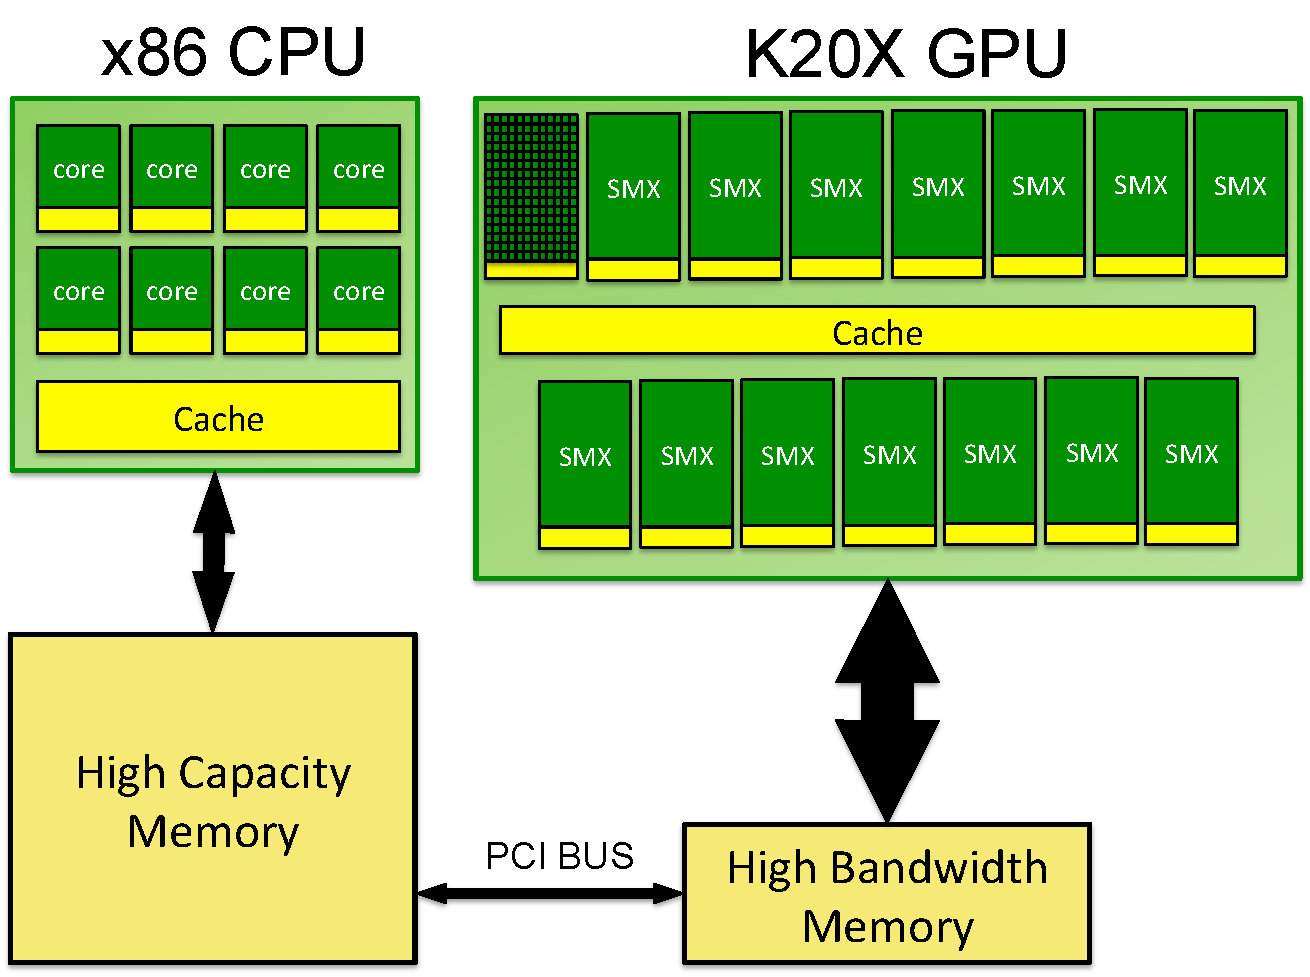
\includegraphics[width=0.9\textwidth]{./images/node.pdf}
    \end{center}
\end{frame}


%%%%%%%%%%%%%%%%%%%%%%%%%%%%%%%%%%%%
\begin{frame}[fragile]{}
%%%%%%%%%%%%%%%%%%%%%%%%%%%%%%%%%%%%
    \begin{info}{Most current applications are not designed for many core}
        \begin{itemize}
            \item exposing sufficient fine-grained parallelism for multi and many core processors is hard
            \item new programming models are required
            \item new algorithms are required
            \item existing code has to be rewritten or refactored
        \end{itemize}
    \end{info}

    \begin{info}{... and compute nodes are under-utilized}
        \begin{itemize}
            \item users are not getting the most out of allocations
            \item the amount of parallelism on-node is only going to increase!
        \end{itemize}
    \end{info}
\end{frame}

%%%%%%%%%%%%%%%%%%%%%%%%%%%%%%%%%%%%
\begin{frame}[fragile]{}
%%%%%%%%%%%%%%%%%%%%%%%%%%%%%%%%%%%%
    \begin{info}{MPI and the free lunch}
        %In 2005 Herb Sutter wrote an article called ``The Free Lunch is Over''
        HPC applications were ported to use the message passing library MPI in the late 90s and early 200s at great cost and effort
        \begin{itemize}
            \item individual nodes with one or two CPUs
            \item break problem into chunks/sub-domains
            \item explicit message passing between sub-domains
        \end{itemize}
        The ``free lunch'' was the regular speedup in codes as CPU clock frequencies increased and as the number of nodes in systems increased
        \begin{itemize}
            \item with little/no effort, each new generation of processor bought significant speedups
        \end{itemize}
    \end{info}

    \centering ...  but there is no such thing as a free lunch
\end{frame}

%%%%%%%%%%%%%%%%%%%%%%%%%%%%%%%%%%%%
\begin{frame}[fragile]{}
%%%%%%%%%%%%%%%%%%%%%%%%%%%%%%%%%%%%
    \begin{info}{How to speed up an application}
        There are 3 ways to increase performance
        \begin{enumerate}
            \item increase clock speed
            \item increase the number of operations per clock cycle
            \begin{itemize}
                \item e.g. vectorization
                \item e.g. multi-core
            \end{itemize}
            \item don't stall
            \begin{itemize}
                \item e.g. cache to avoid waiting on memory requests
                \item e.g. branch prediction to avoid pipeline stalls
            \end{itemize}
        \end{enumerate}
    \end{info}
\end{frame}

%%%%%%%%%%%%%%%%%%%%%%%%%%%%%%%%%%%%
\begin{frame}[fragile]{}
%%%%%%%%%%%%%%%%%%%%%%%%%%%%%%%%%%%%
    \begin{info}{What about just increasing clock frequency?}
        The number of operations per second that can be performed is directly proportional to CPU frequency
        \begin{itemize}
            \item increasing frequency is a great way to increase performance
        \end{itemize}
        Power consumption is a function of frequency $f$
        $$P_{\text{dynamic}}=CV^2f$$
        However voltage $V$ is proportional to frequency, so power increases \emph{super-linearly} with clock frequency
        \begin{itemize}
            \item increasing frequency is an even better way to increase power consumption!
        \end{itemize}
    \end{info}

\end{frame}

%%%%%%%%%%%%%%%%%%%%%%%%%%%%%%%%%%%%
\begin{frame}[fragile]{}
%%%%%%%%%%%%%%%%%%%%%%%%%%%%%%%%%%%%
    \begin{info}{Clock frequency won't increase}
        In fact, clock frequencies have been going down as the number of cores increases
        \begin{itemize}
            \item a 4-core Haswell processor at 3.5 GHz (4*3.5=14 Gops/second) has the same power consumption as a 12-core Haswell at 2.6 GHz (12*2.6=31 Gops/second)
            \item a K20X GPU with 2688 CUDA cores runs at 800 MHz
        \end{itemize}
    \end{info}
\end{frame}

%%%%%%%%%%%%%%%%%%%%%%%%%%%%%%%%%%%%
\begin{frame}[fragile]{}
%%%%%%%%%%%%%%%%%%%%%%%%%%%%%%%%%%%%
    \begin{info}{Parallelism will increase}
        \begin{itemize}
            \item the number of cores in both CPUs and accelerators will continue to increase
            \item the width of vector lanes in CPUs will increase
            \begin{itemize}
                \item currently 4 doubles for AVX
                \item increase to 8 double for AVX-3 (KNL and Skylake)
            \end{itemize}
            \item the number of threads per core will increase
            \begin{itemize}
                \item Haswell supports 2 threads/core
                \item KNL supports 4 threads/core
                \item Power-8 supports 8 threads/core
            \end{itemize}
        \end{itemize}
    \end{info}
\end{frame}

%%%%%%%%%%%%%%%%%%%%%%%%%%%%%%%%%%%%
\begin{frame}[fragile]{}
%%%%%%%%%%%%%%%%%%%%%%%%%%%%%%%%%%%%
    \begin{info}{Memory is slow}
        \begin{itemize}
            \item memory is much slower than processors
            \begin{itemize}
                \item for both CPU and GPU the latency of fetching a cache-line from memory is 100s of cyles
                \item that is 100s of cycles that the processor is stalled, unable to ``work''
                \item latency has to be hidden or reduced to minimise stalling
            \end{itemize}
        \end{itemize}
    \end{info}
    \begin{info}{CPU solution: deep caches and prefetching}
        \begin{itemize}
            \item use fast on-chip memory to \emph{cache} frequently used data
            \item use hardware to \emph{prefetch} data to cache before it is required
        \end{itemize}
    \end{info}
    \begin{info}{GPU solution: over subscribe threads to cores}
        \begin{itemize}
            \item schedule many threads per core
            \item threads that are waiting for data are idle
        \end{itemize}
    \end{info}
\end{frame}

%%%%%%%%%%%%%%%%%%%%%%%%%%%%%%%%%%%%
\begin{frame}[fragile]{}
%%%%%%%%%%%%%%%%%%%%%%%%%%%%%%%%%%%%
    \begin{info}{TLDR: change because power}
        Writing good concurrent code for many-core is difficult
        \begin{itemize}
            \item but the days of easy speed up each generation of CPU are over
            \begin{itemize}
                \item performance gains must not increase power consumption from now on
            \end{itemize}
            \item to continue improving performance many-core will be required
            \item this course will be about one type of many-core architecture NVIDIA GPUs
            \begin{itemize}
                \item both CUDA and OpenACC are GPU-specific
                \item but the concepts will be universally applicable to other many-core architectures (e.g. Xeon Phi)
            \end{itemize}
        \end{itemize}
    \end{info}
\end{frame}

%%%%%%%%%%%%%%%%%%%%%%%%%%%%%%%%%%%%
\begin{frame}[fragile]{}
%%%%%%%%%%%%%%%%%%%%%%%%%%%%%%%%%%%%
    \begin{info}{Terminology}
        \begin{itemize}
            \item the CPU and its memory are called the \emph{host} (because GPUs require a host CPU to coordinate them)
            \item the GPU and its memory are referred to as the \emph{device}
        \end{itemize}
    \end{info}
\end{frame}

%++++++++++++++++++++++++++++++++
\cscschapter{Using GPUs in Your Application}
%++++++++++++++++++++++++++++++++

%%%%%%%%%%%%%%%%%%%%%%%%%%%%%%%%%%%%
\begin{frame}[fragile]{}
%%%%%%%%%%%%%%%%%%%%%%%%%%%%%%%%%%%%
    \begin{info}{Libraries}
        \begin{itemize}
            \item use an off the shelf solution implemented in a library
            \item for specific tasks like dense linear algebra and FFTs, libraries are very hard to beat
            \item e.g. cublas, PETSc, cuFFT
        \end{itemize}
    \end{info}

    \begin{info}{Directives}
        \begin{itemize}
            \item OpenACC and OpenMP 4 define \emph{directives} that can be used to instruct the compiler how to generate GPU code
            \item in theory easy to port codes
        \end{itemize}
    \end{info}

    \begin{info}{GPU-specific Languages}
        \begin{itemize}
            \item languages designed for GPU programming
            \item maximum flexibility and performance
            \item e.g. CUDA and OpenCL
        \end{itemize}
    \end{info}
\end{frame}

\end{document}

